\documentclass[runningheads,a4paper]{llncs}
\usepackage{makeidx}
\usepackage{booktabs}
\usepackage{mathtools}
\usepackage{amsmath}
\usepackage{amsfonts}
% \usepackage{amssymb}
% \usepackage{amsthm}
\usepackage{acronym}
\usepackage{geometry}
\usepackage{hyperref}
\usepackage{float}
\usepackage{graphicx}
\usepackage{cite}

\graphicspath{ {Figures/}{imgs/} }
\begin{document}

\frontmatter

\title{MinCall --- MinION end2end deep learning basecaller}
\author{Neven Miculinić \and Marko Ratković \and Mile Sikić}
\institute{Faculty of
Electrical Engineering and Computing (FER), Zagreb, Croatia}
\maketitle
% \tableofcontents

\begin{abstract}
    The Oxford Nanopore Technologies's MinION is the first portable DNA sequencing device. It's capable of producing long reads, over 100 kBp were reported, however, is has significantly higher error rate than other methods.

    In this study, we created MinCall, an end2end basecaller model for the MinION. The model is based on deep learning and uses convolutional neural networks (CNN) in its implementation. For extra performances is uses cutting edge deep learning techniques and architectures, notably gated residual network, batch normalization and Connectionist Temporal Classification (CTC) loss.

    The best performing 270 layers deep model achieves state-of-the-art 90.5\% match rate on E.Coli dataset using R9 pore chemistry and 1D reads.
\keywords{Basecaller, MinION, R9, CNN, CTC, Next generation sequecing}
\end{abstract}

\section{Introduction}
In recent years, deep learning methods significantly improved the state-of-the-art in multiple domains such as computer vision, speech recognition, and natural language processing \cite{LeCun:1998:CNI:303568.303704}\cite{NIPS2012_4824}.
In this paper, we present application of deep learning in the field of  Bioinformatics for DNA basecalling problem.

Oxford Nanopore Technology's MinION nanopore sequencing platform~\cite{mikheyev2014first} is the first portable DNA sequencing device. It's small weight, of only 90 grams, low capital cost, and long read length combined with high-throughput, real-time data analysis, and decent accuracy yield promising results in various applications. From clinical application such as monitoring infectious disease outbreaks~\cite{judge2015early}\cite{quick2016real}, characterizing structural variants in cancer\cite{norris2016nanopore} and even full human genome assembly~\cite{jain2017nanopore}.

Although MinION is able to produce long reads~\cite{loman1-100k,loman2-800k}, they have a high sequencing error rate. This has been somewhat alleviated with new R9 pore model, replacing older R7 ones. In this paper, we show that this error rate can be reduced by replacing the default base caller provided by the manufacturer with a properly trained neural network model. In the future new R9.5 chemistry and 1D\^2 reads should supersede current models.

In the MinION device, single-stranded DNA fragments move through nanopores, which causes drops in the electric current. The electric current is measured at each pore several thousand times per second, 4000 times exactly in our dataset. The electric current depends mostly on the context of several DNA bases passing through the pore at the time of measurement. As the DNA moves through the pore, the context shifts, and the electric current changes.

The MinION device typically yields reads several thousands bases long, even couple hundred thousand bases long reads were repoted~\cite{loman1-100k,loman2-800k}. However the cost in on accuracy, signicifantly lower than older, more reliable and expensive sequencing methods.

The exact error rate metric is unreliable since multiple pipeline tools could be the issue. First the sample is prepared, hopefully, uncontaminated and matching reference genome as close as possible, then sequenced using the MinION device obtaining raw data. Next, our model (or other groups ones) come along, basecall the sequence. To evaluate error rate metric basecalled read is aligned to the reference genome using aligners with their own errors/biases, mostly commonly used BWA-MEM~\cite{li2013aligning} and Graphmap~\cite{sovic2016fast}.

\section{Background}

\section{Sequencing overview}
Conceptually, the MinION sequencer works as follows. First, DNA is sheared into smaller DNA fragments and adapters are ligated to either end of the fragments. The resulting DNA fragments pass through a protein embedded in a membrane via a nanometre-sized channel, a nanopore. A single DNA strand passes through the pore. Optionally, hairpin protein adapter can merge two DNA strands, allowing both template and complement read passing through the nanopore sequentially for more accurate reads. This technique is referred as 2D reads, while we focus on 1D reads containing only template DNA and no hairpin adapter.

Electrical current runs through the nanopore and exact nucleotides context within influences the nanopore's resistance. This resistive effect is our sensor data, that is the current fluctuations as DNA passes though the pore. The nanopore is 6 nucleotides wide, and many models use this information in their approaches, while we're opted out of this technicality.

\begin{figure}[!ht]
	\begin{center}
		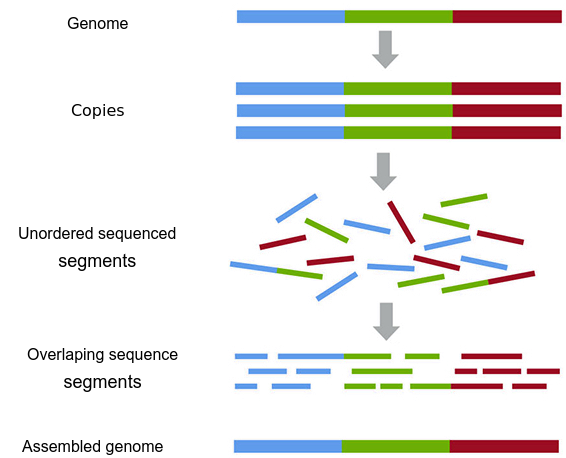
\includegraphics[width=0.6\textwidth]{./imgs/sequencing.png}
		\caption{Depiction of shotgun sequencing}
		\label{fg:sequencing}
	\end{center}
\end{figure}


\begin{figure}[!ht]
	\begin{center}
		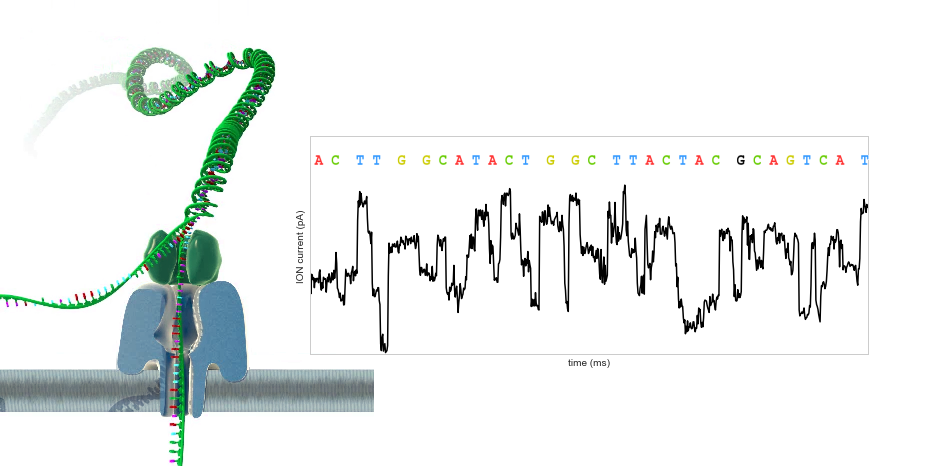
\includegraphics[width=0.7\textwidth]{./imgs/nanopore.png}

		\caption[DNA strain being pulled through a nanopore]{DNA strain being pulled through a nanopore \protect\footnotemark}
		\label{fg:nanopore}
	\end{center}
\end{figure}
\footnotetext{Figure adapted from https://nanoporetech.com/how-it-works}

\section{Basecalling}

The core of the decoding process is the basecalling step. Official basecaller is Metrichor, previously performed in the cloud before being open-sourced under name Nanonet. (Citation, whom?)

Earlier models were (Hidden Markov model) HMM-based where hidden state modeled DNA sequence of length 6 (6-mer) in the nanopore. Pore models were used in computing emission probabilities.~\cite{loman2015complete,schreiber2015analysis,szalay2015novo,timp2012dna} and the recent open source HMM-based basecaller Nanocall~\cite{david2016nanocall}.

Recent models opted using (Recurrent neural network) RNN, notably, DeepNano~\cite{deepnano} and recently open sourced official Nanonet from ONT.

\section{Method}

Instead of opting for the traditional path using HMM or RNN we tried using CNN~(Convolutional neural networks)~\cite{lecun-98}, that is their residual version~\cite{he2016deep}. We opted out for gated residual network variant~\cite{savarese2016learning}. For loss, we used CTC (Connectionist temporal classification)~\cite{graves2006connectionist} between basecalled and the target sequence. The implementation used is open source warp-ctc~\cite{warpctc}. Main computation framework is tensorflow~\cite{tensorflow2015-whitepaper}

\section{Data preprocessing}

Dataset was obtained from (Ask somebody, Marko doesn't know!). In this research, models were trained on the E. Coli K-12 strand. (Should I cite someone for strand). Data was split into train and test subset, such that aligned reads map to different reference genome parts. For initial model data bootstrapping metrichorn was used, version (Ask Someone?).

The fast5 input training files were further split into smaller training blocks, consisting of fixed block size on raw signal. For each block target sequence, basecalled data is used in following way.

We're using basecalled knowledge which tells us on each raw read part which 6-mer were currently in the nanopore. Using this data, we get the intermediate target sequence for each block. To correct for model errors, we use aligned information, that is reference genome and alignment data (cigar string) to correct that information, yielding finalized target sequence. For further performance, we skip first and last training block, since most error aggregate on edges.

Adjacent matching bases are separated with surrogate one, for example, AAA -> AA'A for reasons described in the following section.

\section{Residual arhitecture}

We use gated residual network, that is layer function is like this: $f(x) = k g(x) + x$ Where $x$ is input layer and $k$ constant learnt during training. Specifically, $g$ used is multiple, 1--3 times in our experiments, Relu-BatchNorm-CNN layers.

\section{CTC}

This section gives a brief overview over CTC, for further detail and in depth explanation we recommend original paper~\cite{graves2006connectionist} or searching for contemporary blog posts.

In CTC we have target sequecne $\mathbf{l}$ consisting from symbols of alphabet $\Sigma$. Our models outputs $\mathbf{x}$, and CTC loss maximizes $p(\mathbf{l}|\mathbf{x})$.

$\mathbf{x}$ is consistend of $n$ independent discrete random variables, $X_i$  over domain $\Sigma \cup \text{Blank}$. Path $p$ through $\mathbf{x}$ is assigning for each $X_i$ single value. It's log probabity is $\log P(p) = \sum_i {\log P(X_i=x_i)}$ where $x_i$s define the path.

We further have merging operator on path, $\text{merge}(x_1, x_2, \ldots, x_n)$ which merges together adjacent equivalent elements. For example $\text{merge}(AAAGC) = AGC$.

Then $p(\mathbf{l}|\mathbf{x}) = \sum_{p\in\text{paths}(\mathbf{x}, \text{merged}(p) = \mathbf{l}}{P(p)}$ or less formally, $P(\mathbf{l}|\mathbf{x})$ is sum of all path probabilites which when merged give $\mathbf{l}$

In out concrete $x$ application $\Sigma = \{\text{A G T C A' G' T' A'}\}$

For decoding, we use beam search decoder, with beam width 100.

\section{Results}

\subsection{Final model}

Best performing model used has 270 total layers, divided into 3 90-layer blocks. Between each 90 layers blocks, MaxPool layer is inserted with the receptive width of 2 and stride 2, to ease computation effort and add precision.

Each block consists of 30 gated residual layers, each residual layer composed of 3 sequential Relu-Batch Normalization-Conv1D layers. Each convolutional layer uses the receptive width of 3 with 64 channels as output throughout the model.

\subsection{Performance tables}

As described in the previous section, the model was tested on E.Coli test set and compared to open source Nanonet and Albacore. Albacore doesn't have specific R9 chemistry mode, thus R9.4 was used instead which explains its lower performance on this task. Mean CIGAR operation are in table\ref{table:1} and KDE Match rate plot is in figure~\ref{fig:ecoli_match}.


\begin{table}[h!]
\centering
\begin{tabular}{lrrrrrrr}
\toprule
{} &  Deletion rate &  Error rate &  Insertion rate &  Match rate &  Mismatch rate &  Read length\\
\midrule
albacore     &       0.060 &    0.194 &        0.070 &    0.867 &       0.063 &  9843 \\
nanonet      &       0.088 &    0.190 &        0.040 &    0.897 &       0.062 &  5029 \\
mincall\_m270 &       0.077 &    0.172 &        0.040 &   0.905 &       0.056 &  9378 \\
\bottomrule
\end{tabular}

\caption{Mean performance metrics on E.Coli dataset, 5k sample}
\label{table:1}
\end{table}

\begin{table}[h!]
\centering
\begin{tabular}{lr}
\toprule
{} &  Base pairs/second\\
\midrule
albacore      &      38000 \\
nanonet       &       Slow \\
mincall\_m270 &       3774 \\
\bottomrule
\end{tabular}
\caption{Speed}
\label{table:speed}
\end{table}

\begin{figure}[t]
\centering
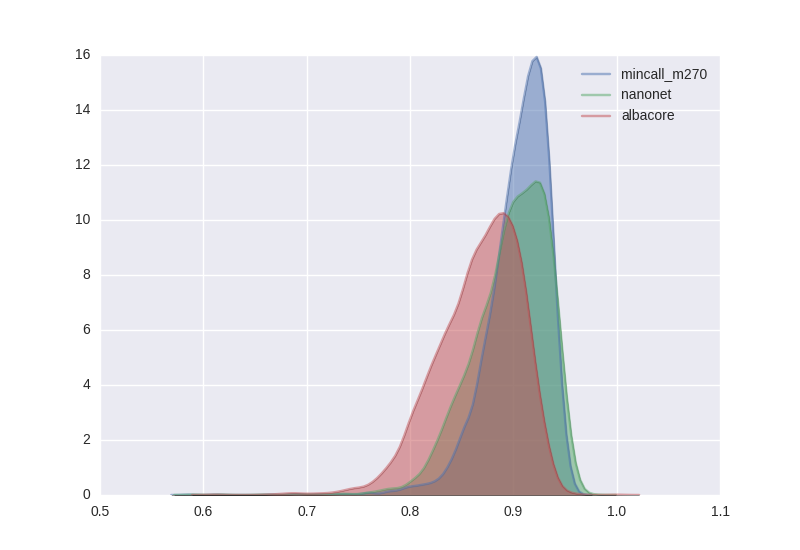
\includegraphics[width=\textwidth]{ecoli_match}
\label{fig:ecoli_match}
\end{figure}


% We also tested and compared models on Human genome~\cite{jain2017nanopore} chromosome Y with R9.4 chemistry. Our model was only trained on R9 chemistry which explain the drop in performance compared to Albacore. In our tests, Nanonet produces significantly shorter read then data length and generally unusable performance on this dataset despite supporting R9.4 chemistry used in the dataset.

\section{Conclusion and further work}

This model used advance state-of-the-art gated residual convolutional neural network, with top models having 270 layers and over 3M parameters, yet improvements over Metrichorn baseline are marginal. As the conclusion, it might be that we've reached Bayesian error rate for R9 chemistry. Furthermore, R9.5 and 1D\^2 reads are under development which shall yield this paper's result obsolete quite soon, yet underlying code developed could easily be adjusted and trained on new data.

Unlike Nanonet which uses custom OpenCL kernels or Albacore --- a novel ONT basecaller as of May 2017 lacking GPU support, this work used world-class computational framework tensorflow with highly optimized kernels and large development community. Therefore resulting paper's effect is showcasing Residual CNN approach or pure CNN approach with CTC loss is marginally better than already established basecaller and providing code in the contemporary framework.

\section{Acknowledgments}

First and foremost I'd like to thank my mentor izv.~prof.~dr.~sc.~Mile Sikić for setting up the problem, guiding us through its beginnings and providing helpful advice for its completion. Next Marko Ratkovic for his not only insightful conversations, but also meaningful code contributions.

Finally, I'm thanking various other people whose code, tools and advice I've used in completing this paper: Fran Jurišić, Ana Marija Selak, Ivan Sović and Martin Šošić.


% set style - not sure which one is official for papers
% spbasic (springer basic makes sense)
\bibliographystyle{spbasic}
% name your BibTeX data base
\bibliography{refs}
\end{document}
